\documentclass[tikz,border=5pt]{standalone}
\usepackage{tikz}
\usetikzlibrary{arrows.meta, positioning, fit}

\begin{document}

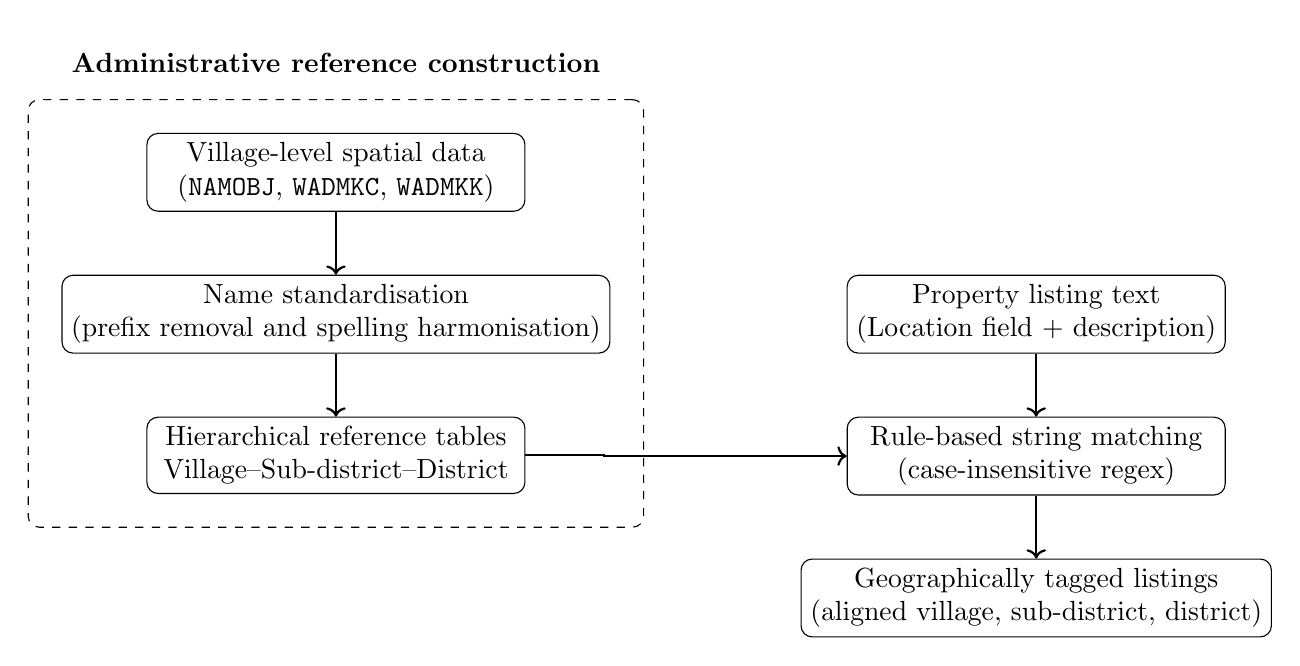
\begin{tikzpicture}[
    every node/.style={
        draw,
        rounded corners,
        align=center,
        minimum width=4.8cm,
        minimum height=9mm
    },
    arrow/.style={->, thick},
    node distance=8mm
]

% ------------------------
% Input spatial reference
% ------------------------
\node (sf) {
Village-level spatial data\\
(\texttt{NAMOBJ}, \texttt{WADMKC}, \texttt{WADMKK})
};

% ------------------------
% Cleaning step
% ------------------------
\node (clean) [below=of sf] {
Name standardisation\\
(prefix removal and spelling harmonisation)
};

% ------------------------
% Reference tables
% ------------------------
\node (refs) [below=of clean] {
Hierarchical reference tables\\
Village--Sub-district--District
};

% ------------------------
% Property listing text
% ------------------------
\node (listing) [right=30mm of clean] {
Property listing text\\
(Location field + description)
};

% ------------------------
% Matching step
% ------------------------
\node (match) [below=of listing] {
Rule-based string matching\\
(case-insensitive regex)
};

% ------------------------
% Output
% ------------------------
\node (output) [below=of match] {
Geographically tagged listings\\
(aligned village, sub-district, district)
};

% ------------------------
% Arrows
% ------------------------
\draw[arrow] (sf) -- (clean);
\draw[arrow] (clean) -- (refs);
\draw[arrow] (listing) -- (match);
\draw[arrow] (refs.east) -- ++(10mm,0) |- (match.west);
\draw[arrow] (match) -- (output);

% ------------------------
% Dashed grouping box
% ------------------------
\node[
    draw,
    dashed,
    rounded corners,
    fit=(sf)(clean)(refs),
    inner sep=12pt,
    label=above:{\textbf{Administrative reference construction}}
] {};

\end{tikzpicture}

\end{document}
